\subsection{画笔设置}
pen 类型函数:
绘制过程中用的是 currentpen,defaultpen。
过程 defaultpen() 返回当前默认画笔属性。
调用过程 resetdefaultpen() 可重设所有画笔默认属性为初始值。
主要属性包括:字体,线宽,颜色,透明度。
默认颜色名如\ref{colors_name}所示:\\
\begin{description}
  \item[颜色:] 默认的颜色有:\\
\begin{figure}[htbp]
\centering
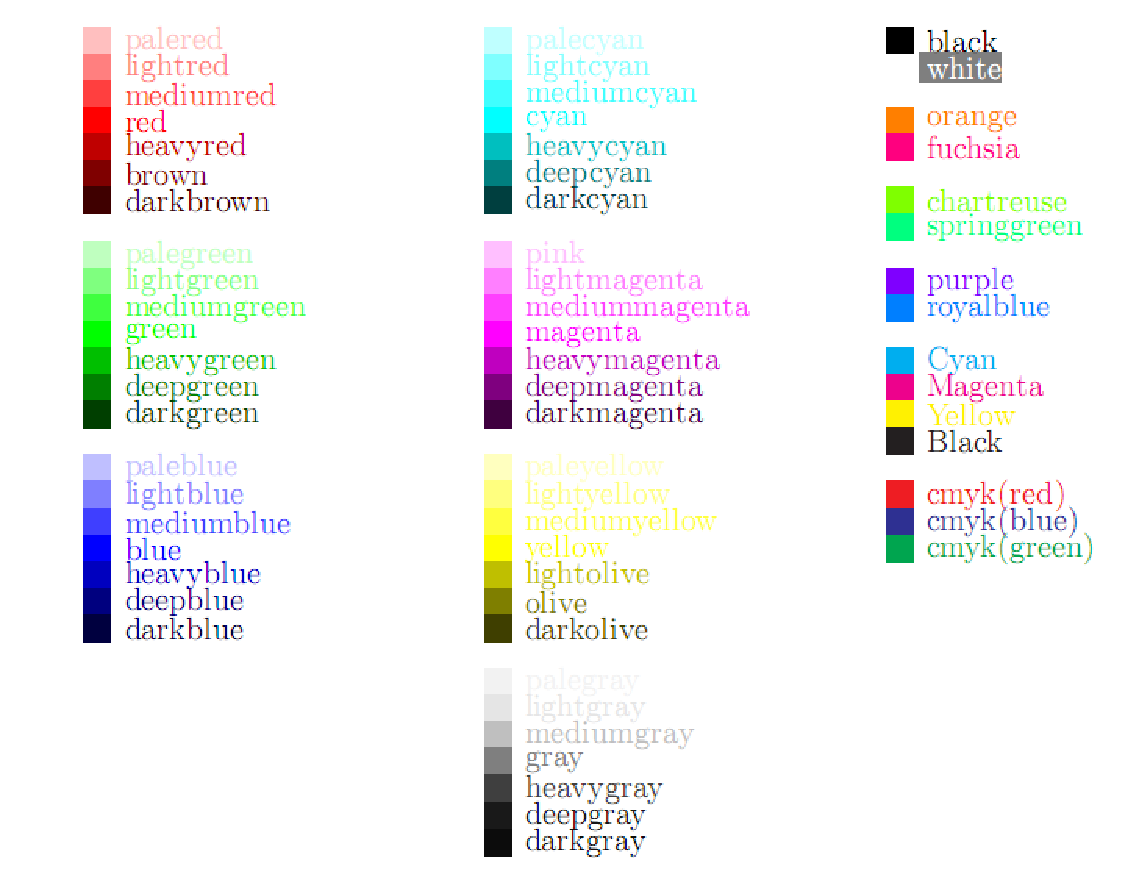
\includegraphics[width=12cm]{colors_name}\\
\caption{asy 各种颜色名称} \label{colors_name}
\end{figure}
  \item[字体:] 默认的字体大小为 12 pt,可以用 defaultpen(pen) 改变。\\
  \fcolorbox{white}{lightgreen}{pen fontsize(real size, real lineskip=1.2*size)}
  \item[线宽:] 默认为 soild 实线类型,0.5dp
  \item[透明度:] opacity 从 0(透明)到 1(不透明)之间先值。
\end{description}
画笔的设置可用如下语句:\\
\fcolorbox{white}{lightgreen}{\parbox{12cm}{
defaultpen(linewidth(0.8)+fontsize(4)+red+opacity(0.5));\\
//设置默认画笔类型\\
pen graypen=linewidth(0.2bp)+gray(0.5);\\
//增加画笔类型
  }}
\clearpage
